\documentclass{beamer}
\usepackage{ctex}
\usepackage[utf8]{inputenc}
\usepackage{graphicx}
\usepackage{amsmath}
\usepackage{amssymb}
\usepackage{booktabs}
\usepackage{hyperref}
\usepackage{subcaption}
\usepackage{multicol}
\usepackage{listings}
\usepackage{multirow}
\usepackage{tabularx}
\usepackage{tikz}

\bibliographystyle{alpha}

\usetheme{Madrid}
\usecolortheme{seahorse}
\setbeamertemplate{caption}[numbered]
% 自定义块颜色
\setbeamercolor{block title}{bg=blue!30,fg=black}
\setbeamercolor{block body}{bg=blue!10,fg=black}
\setbeamercolor{alertblock title}{bg=red!50,fg=black}
\setbeamercolor{alertblock body}{bg=red!20,fg=black}

\title{\textbf{周报}}
\author{向嘉豪}
\institute{衡阳师范学院}
\date{\today}

\begin{document}

\begin{frame}
  \titlepage
\end{frame}

\begin{frame}
  \frametitle{摘要}
  \begin{itemize}
    \item \textbf{论文阅读}:梳理清楚SPHINCS\textsuperscript{+}的所有组件
    \item \textbf{实验}:Python实现WOTS+签名
  \end{itemize}
\end{frame}

\begin{frame}
  \frametitle{SPHINCS\textsuperscript{+} (SPX)}
  \subsection{签名算法初步理解}

  SPX的签名依托Merkle Hash树,将多个安全私钥($sk_i$)视为树的叶子节点,多次哈希后得到根节点($PK$)并对外公开,如图~\ref{fig:spx_sign}所示。对于签名方而言,所有$sk_i$均可使用,但为了保护私钥安全,只会在签名中暴露必须的中间哈希节点与局部私钥。验证方只需据此重构根节点,与公开的$PK$对比一致,即能完成验证。

  \begin{figure}[htbp]
    \centering
    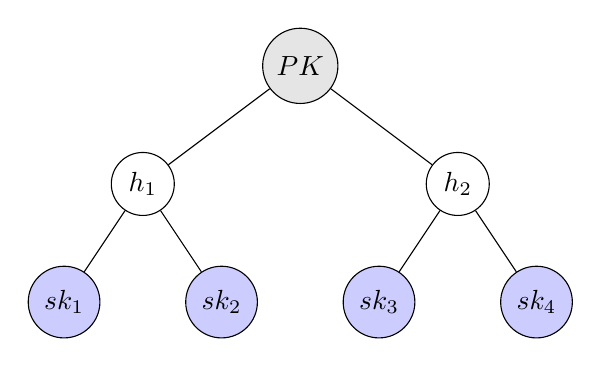
\begin{tikzpicture}[
        level distance=1.5cm,
        level 1/.style={sibling distance=4cm},
        level 2/.style={sibling distance=2cm},
        every node/.style={draw,circle,minimum size=0.8cm}
      ]
      % Root node (pk)
      \node[fill=gray!20] {$PK$}
      % Level 1
      child {node {$h_1$}
        child {node[fill=blue!20] {$sk_1$}}
        child {node[fill=blue!20] {$sk_2$}}
      }
      child {node {$h_2$}
        child {node[fill=blue!20] {$sk_3$}}
        child {node[fill=blue!20] {$sk_4$}}
      };

    \end{tikzpicture}
    \caption{SPX中的Merkle Hash树结构示意图}
    \label{fig:spx_sign}
  \end{figure}
\end{frame}

\begin{frame}
  \frametitle{FORS树}
  FORS(Forest Of Random Subsets)树由$k$个并排的Merkle子树组合而成(图\ref{fig:fors_tree})。每个子树根节点用于拼接形成FORS的签名$SIG_{FORS}$. 在验证环节,需要公开相应私钥部分以及各子树的中间哈希节点,以重建并校验每个子树的根节点。FORS基于消息$m$的哈希值,快速定位并公开对应的$sk_i$,然后将所有子树的根节点拼接成一个整体,用于后续HT树的输入。

  \begin{figure}[htbp]
    \centering
    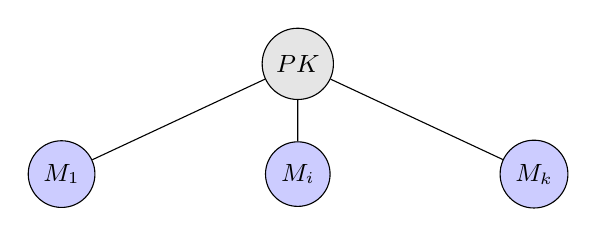
\begin{tikzpicture}[
        level distance=1.4cm,
        level 1/.style={sibling distance=3cm},
        every node/.style={draw,circle,minimum size=0.65cm,font=\small},
        % edge from parent/.style={->,>=stealth,thick}
      ]
      % Root node
      \node[fill=gray!20] {$PK$}
      child {node[fill=blue!20] {$M_1$}}
      child {node[fill=blue!20] {$M_i$}}
      child {node[fill=blue!20] {$M_k$}}
      ;
    \end{tikzpicture}
    \caption{FORS树示意图:$k$个Merkle子树并排组合}
    \label{fig:fors_tree}
  \end{figure}
\end{frame}

\begin{frame}
  \frametitle{HT树}
  HT(Hypertree)结构采用分层聚合的方式(图\ref{fig:ht_tree}):每层XMSS树的根节点作为下一层的叶子节点,最终在顶部生成全局的$PK$. 在验证环节,SPX结合各层子树的WOTS+签名与中间哈希节点来完成验证流程。

  \begin{figure}[htbp]
    \centering
    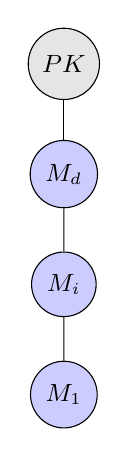
\begin{tikzpicture}[
        level distance=1.4cm,
        level 1/.style={sibling distance=4cm},
        every node/.style={draw,circle,minimum size=0.65cm,font=\small},
      ]
      % Root node
      \node[fill=gray!20,font=\small] {$PK$}
      child {node[fill=blue!20] {$M_d$}
        child {node[fill=blue!20] {$M_i$}
          child {node[fill=blue!20] {$M_1$}}
        }
      };
    \end{tikzpicture}
    \caption{HT树示意图:逐层汇聚得到全局公钥}
    \label{fig:ht_tree}
  \end{figure}
\end{frame}

\begin{frame}
  \frametitle{Python实现WOTS+签名}
  \textbf{实现进度:} 主要包括FORS签名和HT签名,FORS签名依赖于Merkle树的构建和哈希函数的实现,HT签名以XMSS树为基础,同时需要WOTS+签名XMSS树的叶子节点。目前已完成WOTS+签名的Python实现,如图\ref{fig:code_py}所示。
  \begin{figure}
    \centering
    \includegraphics[width=0.3\textwidth]{fig/code_py.png}
    \caption{SPHINCS\textsuperscript{+} Python实现进度}
    \label{fig:code_py}
  \end{figure}
\end{frame}

\begin{frame}
  \frametitle{老师评语}
  \begin{alertblock}{继续推进}

  \end{alertblock}
  \begin{block}{下周计划}
    \begin{itemize}
      \item SPHINCS\textsuperscript{+}的完整实现,包括FORS、HT树等关键组件
      \item 进一步研究SPHINCS\textsuperscript{+}的并行计算特性,探索GPU加速优化方案
    \end{itemize}
  \end{block}
\end{frame}

% 删除: \bibliographystyle{alpha}
% 删除: \bibliography{../../paper}

\end{document}